\chapter{Testowanie płytki}

\section{Płytka i oznaczenia}

\begin{figure}[H]
    \centering
    \includegraphics[scale=0.35]{img/test_plytka/płytka.png}
    \caption{Płytka z oznaczeniami}
    \label{fig:plytka_z_oznaczeniami}
\end{figure}

\begin{center}
    $U_l$ = napiecie na pinie lewym \\
    $U_p$ = napiecie na pinie prawym \\
    $U_{low}$ = napiecie na pinie dla sygnału low \\
    $U_{high}$ = napiecie na pinie dla sygnału high \\
    impulsatory - zmiana przesyłanego sygnału \textbf{low $\xrightarrow{}$ high} oraz \textbf{high $\xrightarrow{}$ low}
\end{center}

\section{Piny}

\begin{itemize}
    \item Zmierzono wartości napięć na pinach \textbf{5V}.
        \begin{gather}
            \label{płytka:U_l} U_l = \textbf{5.02V} \\
            \label{płytka:U_p} U_p = \textbf{5.02V}
        \end{gather}
    \item Następnie sprawdzono działanie impulsatorów używając multimetra do zmierzenia napięcia wyjściowego:
        \begin{figure}[H]
            \centering
                \begin{subfigure}[h]{0.4\textwidth}
                    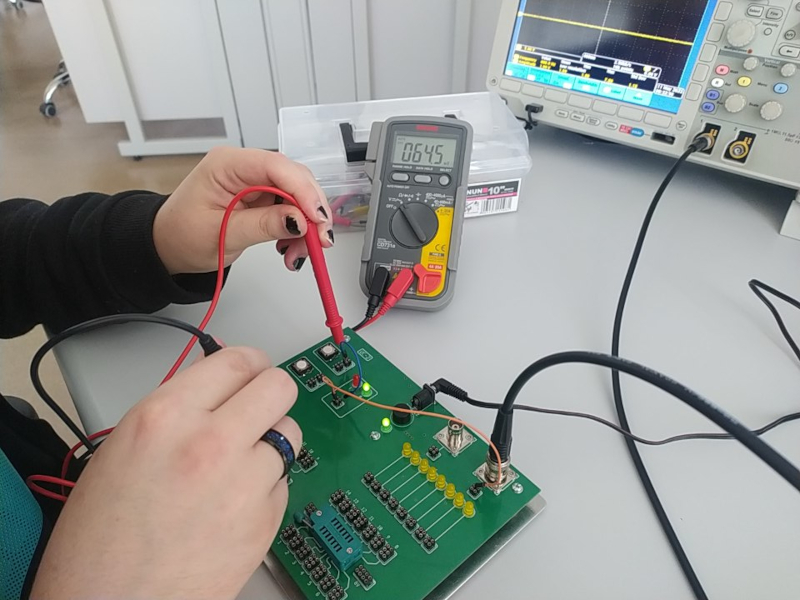
\includegraphics[width=\textwidth]{img/test_plytka/1652306733029_scaled.jpg}
                    \caption*{Pomiar dla $H_{low}$}
                \end{subfigure}
                \begin{subfigure}[h]{0.4\textwidth}
                    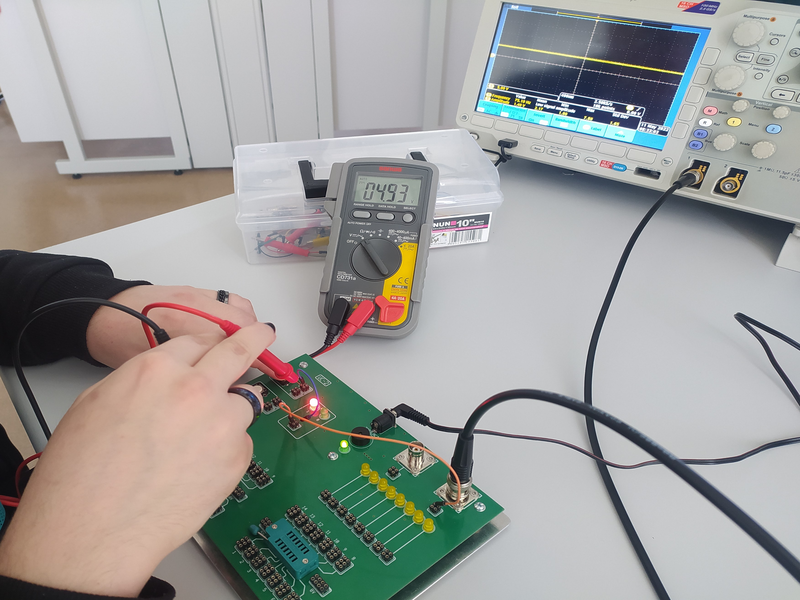
\includegraphics[width=\textwidth]{img/test_plytka/1652306733016_scaled.png}
                    \caption*{Pomiar dla $H_{high}$}
                \end{subfigure}
            \label{płytka:pomiar_impulsatorów}
        \end{figure}
        Zmierzone napięcie wyniosło:
        \begin{gather}
            \label{płytka:U_low} U_{low} = \textbf{0.182V} \\
            \label{płytka:U_high} U_{high} = \textbf{3.525V}
        \end{gather}
        
    \item Za pomocą oscyloskopu sprawdzono sygnał podawany przez impulsator.
        \begin{figure}[H]
            \centering
                \begin{subfigure}[h]{0.45\textwidth}
                    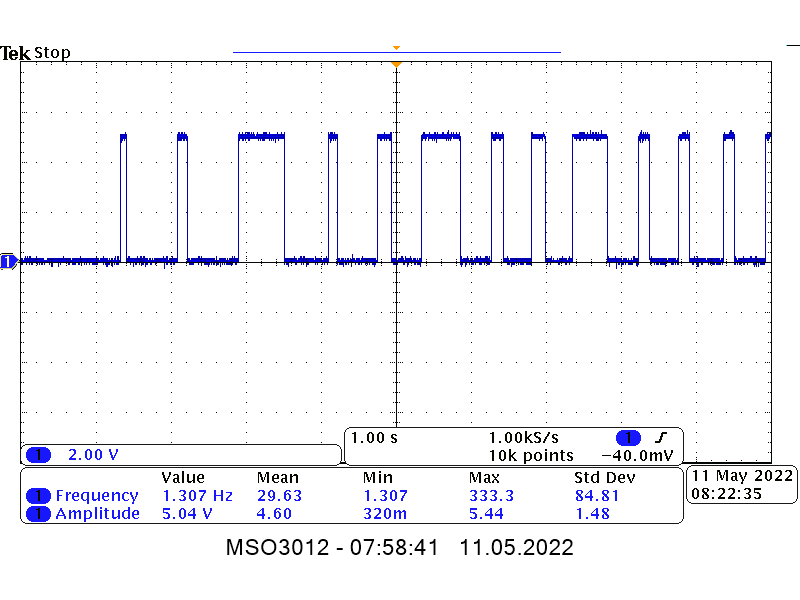
\includegraphics[width=\textwidth]{img/osciloscope/1_dzialajacy_impuls_Q.png}
                    \caption*{Impuls Q ($U_{low} \xrightarrow{} U_{high}$)}
                \end{subfigure}
                \begin{subfigure}[h]{0.45\textwidth}
                    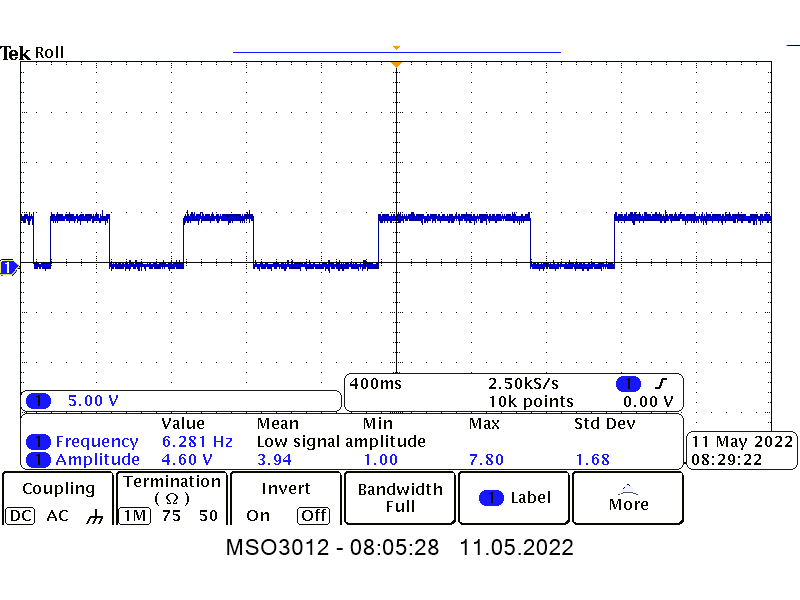
\includegraphics[width=\textwidth]{img/osciloscope/1_dzialajacy_impuls_!Q.png}
                    \caption*{Impuls $\overline{Q}$ ($U_{high} \xrightarrow{} U_{low}$)}
                \end{subfigure}
            \label{płytka:pomiar_impulsatorów_oscyloskop}
        \end{figure}
\end{itemize}

\section{Próbnik stanów logicznych}

\begin{itemize}
    \item Korzystając z impulsatorów sprawdzono działanie próbnika stanów logicznych, poprzez przyłożenie napięcia wyjściowego z impulsatora w stanie $U_H$ oraz $U_L$ do próbnika.
        \begin{figure}[H]
            \centering
            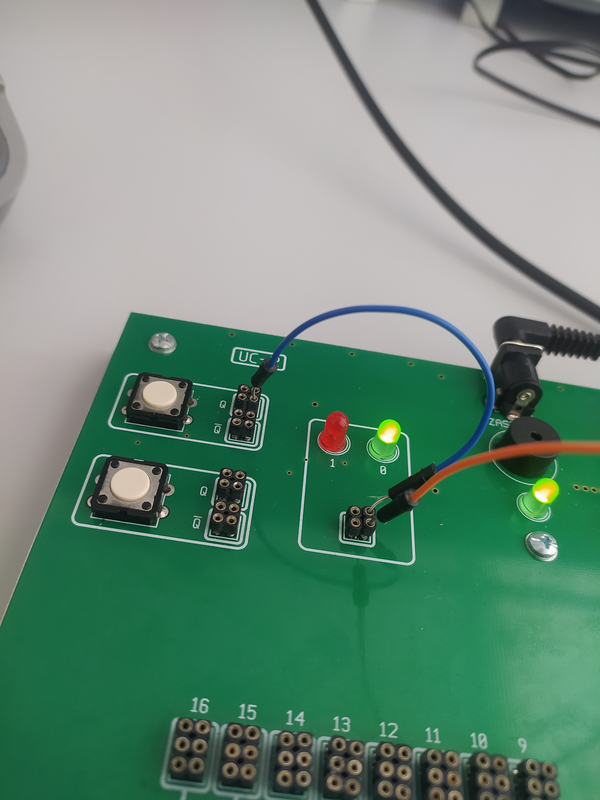
\includegraphics[scale=0.25]{img/test_plytka/1652306733003_scaled.png}
            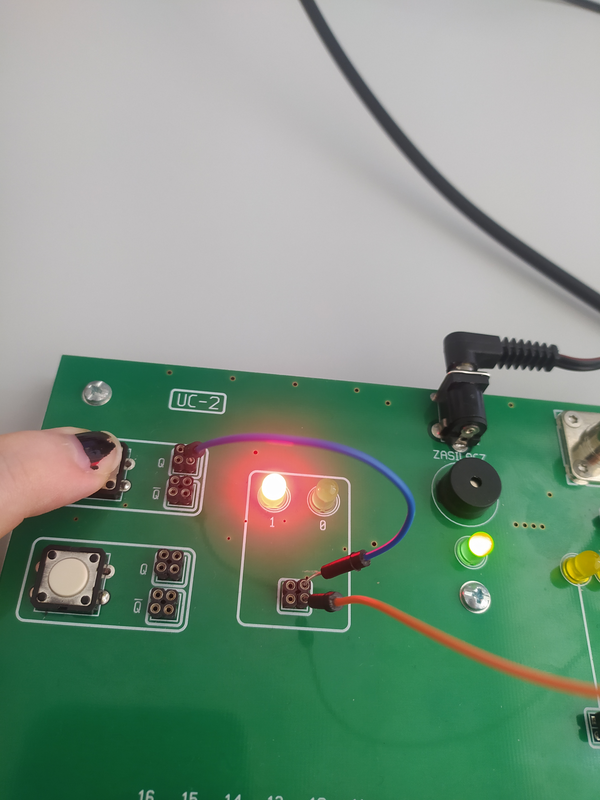
\includegraphics[scale=0.25]{img/test_plytka/1652306732975_scaled.png}
            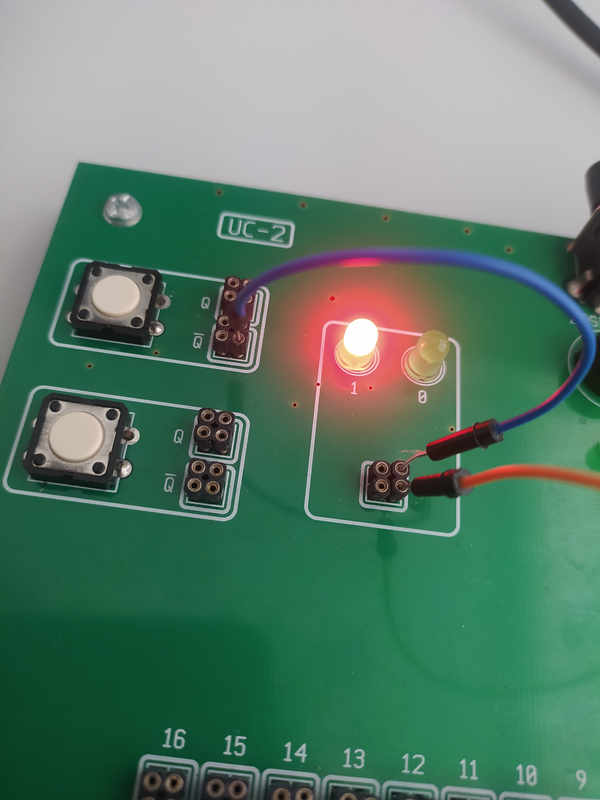
\includegraphics[scale=0.25]{img/test_plytka/1652306732960_scaled.png}
            \caption{Testowanie próbnika stanów logicznych}
            \label{płytka:test_próbnika}
        \end{figure}
    \item Przetestowano działanie zarówno wyjścia \textbf{Q} oraz $\overline{\textbf{Q}}$. Oba działały \textbf{poprawnie}.
\end{itemize}

\pagebreak

\section{Wskaźniki}

\begin{itemize}
    \item Ostatnim testowanym elementem na płytce były wskaźniki, znajdujące się na prawej części płytki.
    \item Wskaźniki testowano poprzez podpinanie wyjścia z impulsatora $\overline{\textbf{Q}}$, które bez wciśniętego impulsatora generuje \textbf{napięcie logicznej jedynki}.
        \begin{figure}[H]
            \centering
                \begin{subfigure}[h]{0.4\textwidth}
                    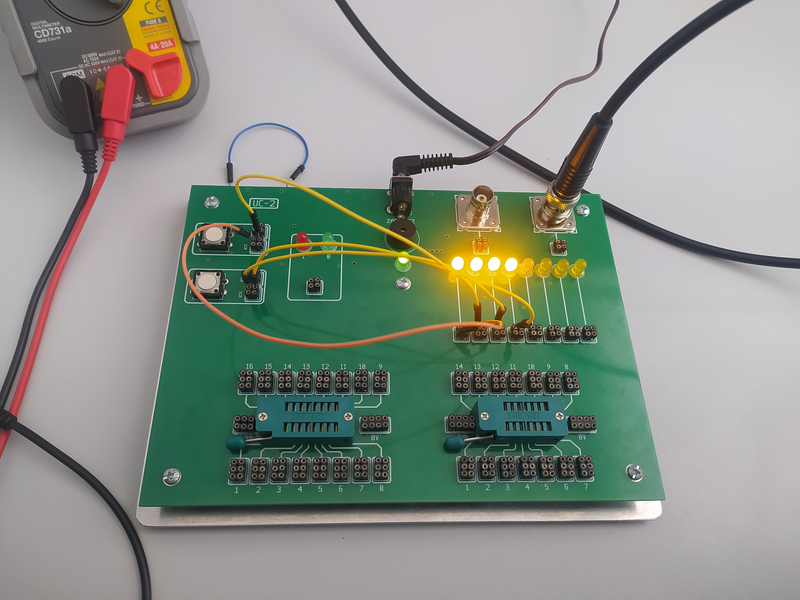
\includegraphics[width=\textwidth]{img/test_plytka/1652306732937_scaled.png}
                \end{subfigure}
                \begin{subfigure}[h]{0.4\textwidth}
                    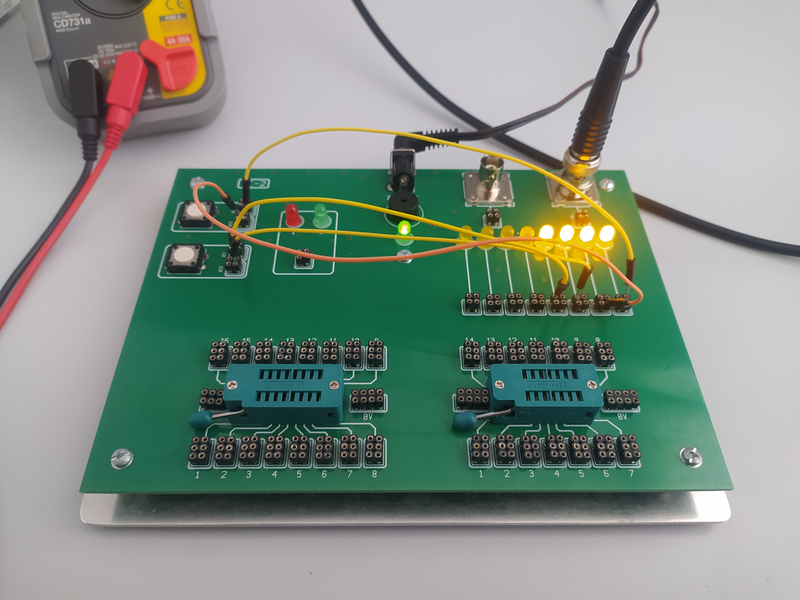
\includegraphics[width=\textwidth]{img/test_plytka/1652306732913_scaled.png}
                \end{subfigure}
            \caption{Działające wskaźniki}
            \label{płytka:test_wskaźników}
        \end{figure}
\end{itemize}

\section{Poprawność działania płytki}

\begin{itemize}
    \item Wskazania na multimetrze (\ref{płytka:U_low}, \ref{płytka:U_high}, \ref{płytka:U_l}, \ref{płytka:U_p}) \textbf{zgadzały} się z przewidywanymi wartościami.
    \item Impulsatory działały \textbf{poprawnie} (\ref{płytka:test_wskaźników})
    \item Próbnik stanów logicznych \textbf{poprawnie} reagował na podawane napięcia z impulsatorów (\ref{płytka:test_próbnika})
    \item Wskaźniki \textbf{poprawnie} reagowały na podawane napięcia (\ref{płytka:test_wskaźników})
\end{itemize}